

\partabstractfp{进程资源是如何处理的?进程与进程间是怎样的关系?进程死亡后会不会内存泄露?不同生命周期下进程资源的处理方式有什么差异?}
\partabstractrp{注:本章的架构是我根据讲课记录自己的理解划分的,可能与讲课不一致,如有错误欢迎指正。子死父收尸章节应该是第一天讲的,为了保持架构的一致性,把它挪到此处进行处理。}
\partabstractlettrine{L}{inux进程出生到死亡,生,死,睡过程} % the first word of the abstract

\part{进程课第2天}

\chapter{进程出生}
\section{进程出生时资源处理}
fork出子进程后,子进程的资源就直接从父进程的进程结构task\_struct拷贝出同样的信息,如\ref{child_fork_task_struct}所示。进程P2刚创建后,其资源是一模一样的。

\begin{figure}[H]
 \wdfigbox
  {\caption{fork子进程资源拷贝}\label{child_fork_task_struct}}
  {
  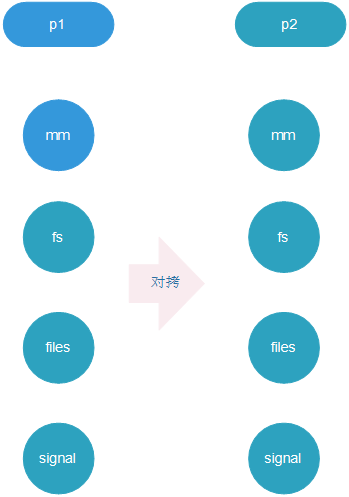
\includegraphics[width=8cm]{./figure/child_fork_task_struct.png}
  \floatfoot{注:所有资源结构体都进行拷贝  }
  }
\end{figure}
之后随着进程变化,本着谁修改谁分裂的原则进行资源变化的处理。

\section{进程分裂时的资源变化 -- COW}
父子进程刚诞生时所得到的资源是一样的,那这些资源在何时发生变化,以及变化后有什么影响,这就涉及到了linux的copy-on-write技术,下面通过 具体的实例来说明父子进程的资源变化流程。\\
COW(copy-on-write)技术是进程fork时采用的,涉及到虚拟内存和实际内存的映射关系。采用了COW技术后,进程处理会有一些现象需要重点注意。比如fork之后的父子进程读写同一个全局变量时,一个变量在不同的进程会显示出不同的值。
\subsection{COW 现象代码}
\begin{lstlisting}[language={C}]
#include <stdio.h>
#include <sys/types.h>
#include <unistd.h>
int data = 10;
int child_process()
{
    printf("child process %d, data %d\n", getpid(), data);
    data = 20;
    printf("child process %d, data %d\n", getpid(), data);
    _exit(0);
}
int main(int argc, char * argv[])
{
    int pid;
    pid = fork();
    if(pid == 0){
        child_process();
    }
    else{
        sleep(1);
        printf("parent process %d, data %d", getpid(),data);
        _exit(0);
    }
    return 0;
}
\end{lstlisting}
在正常情况下,程序修改全局变量data,再打印data,会是修改后的值 20,代码中子进程修改全局变量为20后,父进程等待1s,确保子进程已修改完成,但父进程最终打印的结果还是10。
\begin{latexcmd}[label= COW现象]
#运行程序的显示结果如下
child process 9491, data 10
child process 9491, data 20
parent process 9490, data 10
\end{latexcmd}

下面我们具体分析程序背后采用COW的原理和流程。\\
\subsection{COW 实现技术原理}
fork进程前后的内存关系如\ref{linux_fork_mem_compare}所示,
\begin{description}
  \item[\heiti{fork前第1阶段:}] 全局变量data对应数据段内存vir和phy都在数据段,权限为可读可写。
  \item[\heiti{fork后:}] vir和Phy的权限全部变成只读权限,读内存正常,写内存会进入page fault缺页中断。
  \item[\heiti{fork后写内存:}] 写内存后,发生缺页中断,Linux会重新申请一个4k内存,将新物理内存指向更改了内存地址的进程vir。同时将老的4k内存拷贝给新的内存,同时将权限改为R+W,这样父子进程的同一个vir虚拟地址就分别对应2个独立的可读可写的物理地址。总之谁先写谁拿到新的物理内存,原内存留给剩下的进程。
\end{description}
\begin{figure}[H]
 \wdfigbox
  {\caption{fork进程前后内存映射关系}\label{linux_fork_mem_compare}}
  {
  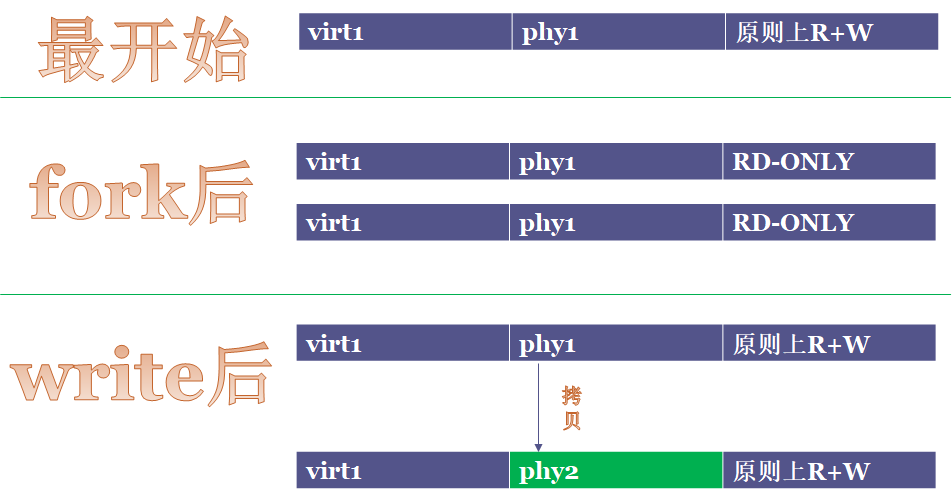
\includegraphics[width=9cm]{./figure/cow_fork_virmem_compare.png}
  \floatfoot{注:第一列为虚拟地址,第二列为物理地址,最后一列对应内存的读写权限 }
  }
\end{figure}
\subsection{无法用COW的情况:VFORK}
COW技术必须借助MMU(内存管理单元)来实现。COW是通过改变虚拟内存和物理内存的映射关系来实现,没有MMU的系统,无法实现虚拟内存和物理内存的映射。也无法调用fork函数,无MMU系统对应调用的是vfork函数,其资源变化对比fork如\ref{vfork_mem}所示:
\begin{figure}[H]
 \wdfigbox
  {\caption{vfork进程内存}\label{vfork_mem}}
  {
  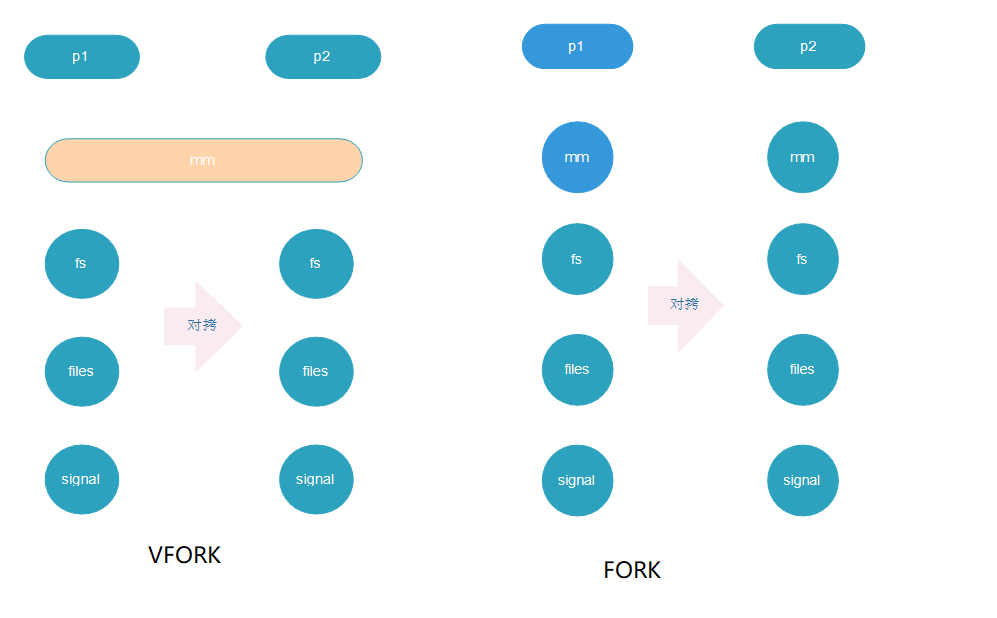
\includegraphics[width=10cm]{./figure/vfork_mem.png}
  \floatfoot{注:mm为同一份,没有进行拷贝  }
  }
\end{figure}
vfork的特点:vfork会阻塞父进程,只有等子进程完全退出后才执行父进程。vfork特性演示视频如下所示:

\begin{tcolorbox}[colback=blue!5,colframe=blue!75!black,title=vfork 视频]
\videoattach{2- vfork.avi}{vfork与COW区别}{https://share.weiyun.com/5G2jlaC}
\end{tcolorbox}

\subsection{强制共享资源--线程}
当P1和P2都用同一个资源,资源结构体不进行拷贝,P2的资源指针直接指向P1,这样就体现出线程的特征:可以调度又共享一样的资源。Linux中也是这样来实现线程的,调用pthread\_create时,会调到CLONE的API,这样就会让P2的资源指针指向P1。
\begin{figure}[H]
 \wdfigbox
  {\caption{线程资源处理}\label{thread_mem}}
  {
  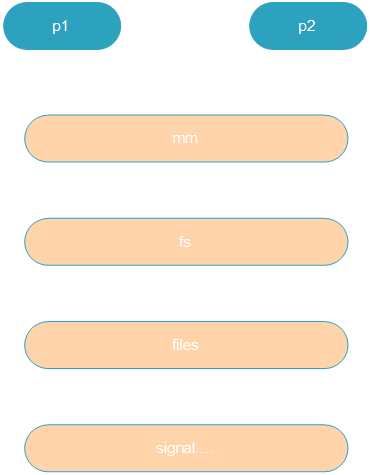
\includegraphics[width=4cm]{./figure/thread_resource.png}
  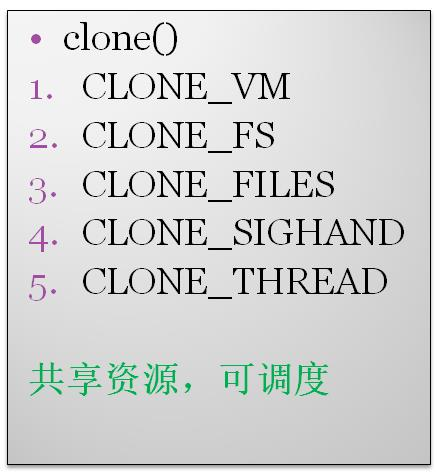
\includegraphics[width=4cm]{./figure/clone_api.jpg}
  \floatfoot{注:最终调用的API为CLONE,pthread\_create  }
  }
\end{figure}
\begin{tcolorbox}[colback=blue!5,colframe=blue!75!black,title=thread 视频]
\videoattach{3- thread.avi}{thread视频演示}{https://share.weiyun.com/5EsHhl5}
\end{tcolorbox}

\section{第1个进程,进程0与进程1}
开机后进程0创建出进程1,开机后进程0会退化成idle进程,idle进程的优先级最低。此进程运行的原则是所有其他的进程不运行时它就开始运行,当运行idle进程时,cpu就设置成低功耗模式。(注:与开机键中的suspend的区别是idle状态时只有cpu是低耗,suspend时显示器电源等其他设备也会进入低功耗)。此设计的精妙之处在于,如果不用进程0,进程进入低功耗模式的判断标准就变成了所有进程退出后要检查一下是否是最后一个进程,如果是最后一个就进入低功耗模式。这样的设计就会把检查状态耦合到了每个进程之中。增加进程0设计的好处在于,设计就简化只要判断是否在idle进程就可以了。实现了去耦合。
视频演示如下:
\begin{tcolorbox}[colback=blue!5,colframe=blue!75!black,title=idle进程视频]
\videoattach{7- idle-process.avi}{idle进程视频演示}{https://share.weiyun.com/5et9Oz8}
\end{tcolorbox}

\chapter{进程运行}
~\\程序运行时大部分进程状态为运行或睡眠。调度算法解决可以跑的运行状态(就绪和运行),剩下的不可以跑的进程就是睡眠和等待。睡眠实现对应的代码就是调用了schdule函数,唤醒则是对应的是schdule返回。一个进程等资源就会去睡,linux所有的睡眠,对应的task\_struct就会挂在队列wait\_queue上,当资源来了后,就会唤醒等待队列上的进程。视频演示如下:
\begin{tcolorbox}[colback=blue!5,colframe=blue!75!black,title=等待队列视频]
\videoattach{6- sleep-waitqueue.avi}{进程等待队列视频演示}{https://share.weiyun.com/53SMfMt}
\end{tcolorbox}


\chapter{进程死亡}
fork执行后,就会变成2个进程返回,而不是一个进程返回两次。两个进程用的是同一段代码,不同的是在判断fork的返回值后会走向不同的分支。子进程返回的是0,则if(pid == 0)后执行的是子进程,父进程接收到的返回值是子进程的pid值。如下所示:

\dirtree{%
.1 fork之后.
.2 返回值为-1\DTcomment{fork失败}.
.2 返回值为0\DTcomment{子进程返回}.
.2 返回值为pid号\DTcomment{父进程返回}.
}

\section{子死父收尸}
linux中子进程死亡时首先变成僵尸,父进程通过wait来获取子进程的死亡原因。调用的API如\ref{child_wait}所示,父进程通过分析子进程的退出码就可以知道具体的退出原因了。

\begin{figure}[H]
 \wdfigbox
  {\caption{子进程死亡原因获取}\label{child_wait}}
  {
  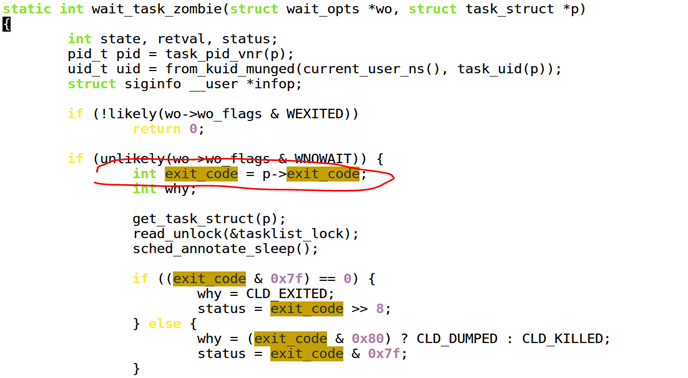
\includegraphics[width=10cm]{./figure/child_wait.png}
  \floatfoot{父进程通过exit\_code获取子进程退出信息}
  }
\end{figure}

\begin{tcolorbox}[colback=blue!5,colframe=blue!75!black,title=子进程死亡原因获取视频]
\videoattach{1- child-waited-by-parent.avi}{父进程获取子进程死亡原因视频演示}{https://share.weiyun.com/5FwLvlt}
\end{tcolorbox}
\section{父死子托孤}
任何一个进程死亡后有个原则,首先托付给subreaper,如果没有subreaper则托付给init。如\ref{child_process_died}所示。进程可以通过API来设置自己为subreaper。subreaper要注意调用wait来处理可能托付过来的僵尸进程。
\begin{figure}[H]
 \wdfigbox
  {\caption{进程死亡后挂接关系}\label{child_process_died}}
  {
  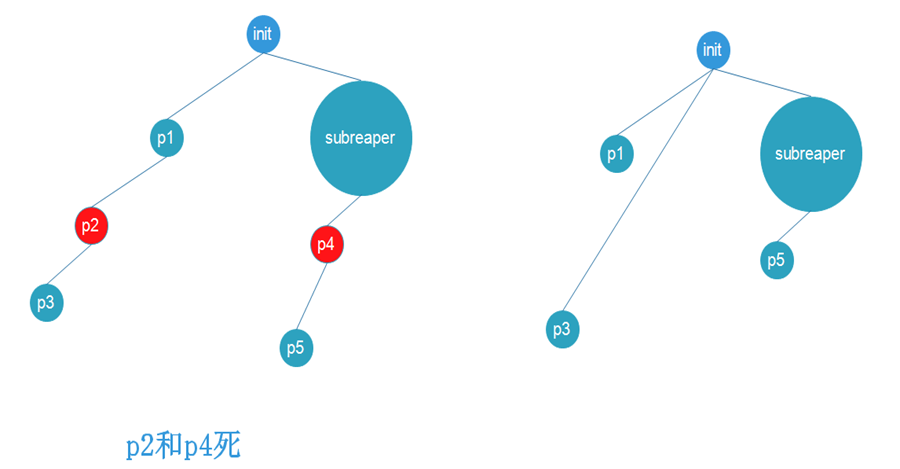
\includegraphics[width=10cm]{./figure/child_process_died.png}
  \floatfoot{挂到init或subreaper  }
  }  
\end{figure}

\begin{tcolorbox}[colback=blue!5,colframe=blue!75!black,title=进程托孤视频]
\videoattach{5- orphan.avi}{进程托孤视频演示}{https://share.weiyun.com/57CLGS4}
\end{tcolorbox}
\clearpage
%%% Local Variables:
%%% TeX-master: "main"
%%% End:

